\documentclass[3pt,landscape]{article}
%ss[10pt,landscape]{article}
\usepackage{multicol}
\usepackage{calc}
\usepackage{ifthen}
\usepackage[landscape]{geometry}
\usepackage{amsmath,amsthm,amsfonts,amssymb}
\usepackage{color,graphicx,overpic}
\usepackage{wrapfig}
\usepackage{hyperref}
\usepackage[shortlabels]{enumitem}


\pdfinfo{
/Title (final.pdf)
/Creator (TeX)
/Producer (pdfTeX 1.40.0)
/Author (Eddie Groshev)
/Subject (Foundations of Computer Graphics)
/Keywords (pdflatex, latex,pdftex,tex)}

% This sets page margins to .5 inch if using letter paper, and to 1cm
% if using A4 paper. (This probably isn't strictly necessary.)
% If using another size paper, use default 1cm margins.
\ifthenelse{\lengthtest { \paperwidth = 11in}}
    { \geometry{top=.3in,left=.3in,right=.3in,bottom=.3in} }
    {\ifthenelse{ \lengthtest{ \paperwidth = 297mm}}
        {\geometry{top=1cm,left=1cm,right=1cm,bottom=1cm} }
        {\geometry{top=1cm,left=1cm,right=1cm,bottom=1cm} }
    }

% Turn off header and footer
\pagestyle{empty}

% Redefine section commands to use less space
\makeatletter
\renewcommand{\section}{\@startsection{section}{1}{0mm}%
                            {-1ex plus -.5ex minus -.2ex}%
                            {0.5ex plus .2ex}%x
                            {\normalfont\large\bfseries}}
\renewcommand{\subsection}{\@startsection{subsection}{2}{0mm}%
                            {-1explus -.5ex minus -.2ex}%
                            {0.5ex plus .2ex}%
                            {\normalfont\normalsize\bfseries}}
\renewcommand{\subsubsection}{\@startsection{subsubsection}{3}{0mm}%
                            {-1ex plus -.5ex minus -.2ex}%
                            {1ex plus .2ex}%
                            {\normalfont\small\bfseries}}
\makeatother

% Define BibTeX command
\def\BibTeX{{\rm B\kern-.05em{\sc i\kern-.025em b}\kern-.08em
    T\kern-.1667em\lower.7ex\hbox{E}\kern-.125emX}}

% Don't print section numbers
\setcounter{secnumdepth}{0}


\setlength{\parindent}{0pt}
\setlength{\parskip}{0pt plus 0.5ex}

%My Environments
\newtheorem{example}[section]{Example}
% -----------------------------------------------------------------------

\def\ci{\perp\!\!\!\perp}

\begin{document}
\raggedright
\footnotesize
\begin{multicols}{3}


% multicol parameters
% These lengths are set only within the two main columns
%\setlength{\columnseprule}{0.25pt}
\setlength{\premulticols}{1pt}
\setlength{\postmulticols}{1pt}
\setlength{\multicolsep}{1pt}
\setlength{\columnsep}{2pt}

\begin{center}
    \Large{\underline{CS 184 MT1 Note Sheet}} \\
\end{center}

%Maximum likelihood estimation
%CHECK - Decision theory
%CHECK - Multivariate Gaussians
%CHECK - Linear/quadratic discriminant analysis
%CHECK - Linear regression
%CHECK - Logistic regression
%CHECK - Loss Functions (hinge loss, log loss, misclassification loss)
%CHECK - Optimization (Gradient descent, Newton's Method, Lagrange multipliers)
%CHECK - SVMs (primal, dual)
%Kernels
%CHECK - Nearest neighbour

\subsection*{Color}
{\bf Light}: Electromagnetic radiation between 400nm and 700nm.
{\bf Spectral} color (monochromatic): Light at a single frequency.\\
%Spectral color are bright and distinct in appearance
{\bf ROYGBIV}\(\rightarrow\) Red Orange Yellow Greeen Blue Indigo Violet\\
Most visible colors are a mix of several frequencies.\\
Eyes don't ``see" spectrum or intensity values.\\
Eyes make limited measurements, eyes and brain both adapt to circumstances. Everything is relative.\\
%Look at True/False problems regarding relativity
%Mach Bands: exaggerate the contrast between edges of slightly differing shades of gray, as soon as they contact one another.
{\bf Bezold Effect}: Colors outlined in white/black appear lighter/darker.
\begin{multicols}{2}
\center
Cones\\
-Less sensitive\\
-Light adjusted (Photopic)\\
-Short, Medium, Long\\
-Concentrated in fovea (center of retina)\\
\columnbreak
Rods:\\
-More sensitive\\
-Dark adjusted (Scotopic)\\
-Spread over the retina.\\
-Contribute to (bluish) color perception
\end{multicols}
%Rod response curve is between medium and short.
{\bf Trichromaticity}: eye records color by 3 measurements.\\
\(L = \int\Phi(\lambda)L(\lambda)d\lambda\), 
\(M = \int\Phi(\lambda)M(\lambda)d\lambda\), 
\(S = \int\Phi(\lambda)S(\lambda)d\lambda\)\\
{\bf Metamers}: Different light spectrums produce same cone response\\
Cone response is linear: \(n\Phi_1+\Phi_2 \implies nL_1+L_2\)\\
{\bf Additive Mixing}: Given any 3 primaries \(p_1,p_2,p_3\), match \(\Phi\) with \(\alpha p_1 + \beta p_2 + \gamma p_3\)\\
%Color matching functions?
%Imaginary set of primaries with positive values, XYZ
{\bf Gamut}: convex full of the primary chomaticities\\
Gamut of CIE 1931 (XYZ) primaries encompasses the whole horseshoe.\\
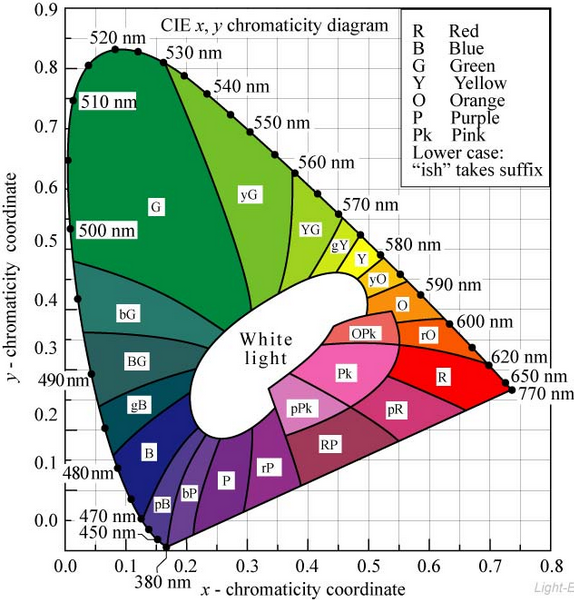
\includegraphics[scale=0.4]{images/gamut}\\
{\bf Subtractive Mixing}: Given any 3 primaries \(p_1,p_2,p_3\), match \(\Phi\) with \(W-(\alpha p_1 + \beta p_2 + \gamma p_3)\). Black is usually used to save ink.\\
%Color Spaces: RGB, HSV: HueSaturationValue
%Monitors map pixel values to intensity levels, but are not linear.
%Monitor nonlinearity characterized by exponential function I=a^\gamma
%I is monitor intensity, a is pixel value, and gamma is some tuned parameter
%To find gamma, make a patch of 0.5 monitor intensity (alternate white/black)
%Dynamic Range: max/min monitor values are limited
%Tone Mapping: Map one set of colors to another
%Reflection: Some frequencies bounce off others absorb
%Transmission: Some frequencies pass through, others reflect/absorb
%Scattering: Interaction with small particles in medium, short wavelengths scatter.
%Interference: Cancelation/Reinforcement between light waves
%Iridescence: Interaction of light with small structures and thin transparent surfaces.
%Fluorescence: Emission of photon at another frequency
%Black Body Radiation: Energy radiated by hot objects, emitted frequency is temperature dependent. Notion of "color temperature".
%\(E(\lambda)\propto\frac{1}{\lambda^5}(\frac{1}{exp(hc/k\lambda T)-1}) \)

\subsection*{Shading}
{\bf Local Shading}: shading considered in isolation.\\
{\bf Non-local}: shadows, reflections, refraction, indirect lighting\\
{\bf BRDF}: Bi-directional Reflectance Distribution Function\\
BRDF defines how light is reflected at an opaque surface.\\
BRDF is frequency dependent.\\
BRDF doesn't capture Subsurface Scattering (BSSRDF)\\
%BRDF is the spatial variation capture by "the material"
Approximate BRDF as sum of Ambient, Diffuse, and Specular components.\\
Diffuse: matte (Lambertian) surface reflectance depends on cosine of angle between surface and light direction.\\
Specular: Mirror-like reflection (Phone Illumination Model) depends on view direction. \(\hat{r}=-\hat{l}+2(\hat{n}^T\hat{l})\hat{n}\)\\
``Half-angle'' approximation: \(k_sI(\hat{h}^T\hat{n})^p\) where \(\hat{h}=\frac{\hat{l}+\hat{v}}{||\hat{l}+\hat{v}||}\)\\
Ambient: Accounts for omnifirectional light.\\
\boxed{R = k_aI + k_dI\max(\hat{n}^T\hat{l}, 0) + k_sI\max(\hat{r}^T\hat{v}, 0)^p}\\
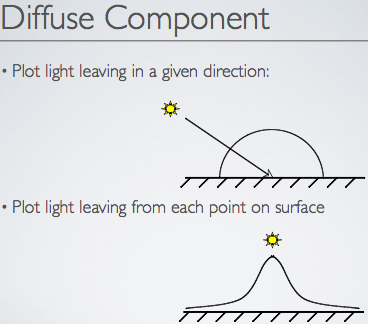
\includegraphics[scale=0.32]{images/diffuse}
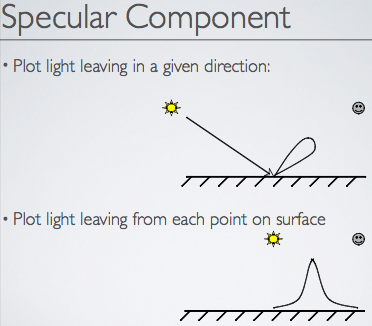
\includegraphics[scale=0.32]{images/specular}\\
Metal specular reflects its color, plastic specular reflects as white.\\
{\bf Anisotropic}: Reflection depends on direction relative to material.\\
{\bf Point Light}: Direction changes over surface\\
{\bf Directional Light}: Constant direction (point light at infinity)\\
{\bf Falloff}: \(1/r^2\) looks bad. Use \(1/r\) instead\\
{\bf Flat Shading}: Constant normal per triangle/polygon.\\
{\bf Gouraud Shading}: Compute shading at each vertex. Type of smooth shading (where normals/colors are interpolated), fast, terrible for specular reflections.\\
{\bf Phong Shading}: Compute shading at each pixel. Type of smooth shading, expensive.\\
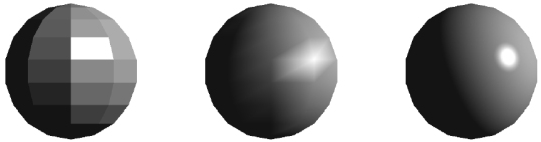
\includegraphics[scale=0.4]{images/shading}\\

\subsection*{Transformations}
%{\bf Mapping Function}: Maps points in original image p=(x,y) to points in transformed image p`=(x`,y`)\\ 
%Shears are linear geometric.
%Swirls are non-linear geometric.
%Edge finding is color space transform.
%{\bf Instancing}: Reuse geometric description, with different transform.
%Composing two linear functions gives a linear function. We transform polygons by transforming vertices. Interior is defined by interpolation of vertices.
{\bf Rotations}: Preserve lengths and distance to origin, are orthonormal, det(R)=1, positive\(\rightarrow\)counter-clockwise. (In 2D ONLY, pure rotations commute)\\
In general matricies are associative, but not commutative.\\
{\bf Scales}: Diagonal matricies, negative values flit, axis aligned scales\\
{\bf Shears}: Composition of rotations and scales\\
{\bf SVD}: Any matrix can be writen as \(A=QSR^T\) where Q and R orthonormal and S diagonal.\\
{\bf Polar Decomposition}: \(A=PRSR^T\) where \(P=QR^T\)\\
{\bf Homogeneous Coordinates}: Append 1/0 at the end of the direction/point vectors. Used for translations and projections.\\
Normals do not transform normally. Given transformation M, \(n_{new}=(M^{-1})^Tn_{old}\)\\
\(R_x = 
\begin{bmatrix}
1 & 0 & 0 \\
0 & \cos(\theta) & -\sin(\theta)\\
0 & \sin(\theta) & \cos(\theta)
\end{bmatrix}
R_y = 
\begin{bmatrix}
\cos(\theta) & 0 & \sin(\theta) \\
0 & 1 & 0\\
-\sin(\theta) & 0 & \cos(\theta)
\end{bmatrix}\)
\(R_z = 
\begin{bmatrix}
\cos(\theta) & -\sin(\theta) & 0 \\
\sin(\theta) & \cos(\theta) & 0\\
0 & 0 & 1
\end{bmatrix}
\)\\
{\bf Euler Angles}: Allow tumbling, Non-unique, Gimbal-lock, built from axis-aligned matricies \(R=R_zR_yR_x=rot(x,y,z)\)
{\bf Exponential Maps}: Encode the rotation-axis and rotation amount as a vector \(\hat{r}\) where \(\theta = |\hat{r}|\). Allows tumbling, no gimbal-lock, singularity on shells at 2\(\pi\)\\
%TODO: Replace the picture below, with formulas
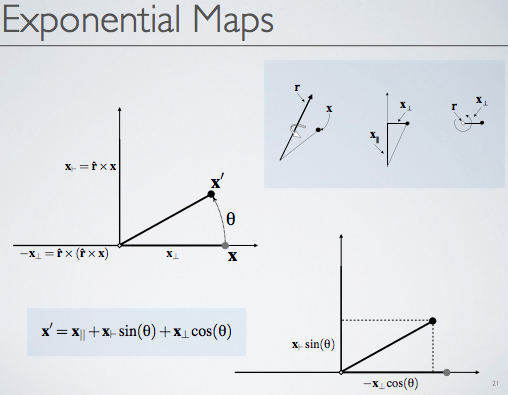
\includegraphics[scale=0.5]{images/exponential_map}\\
{\bf Rodriguez Formula}: \(x^{'}=\hat{r}(\hat{r}\cdot x)+\sin(\theta)(\hat{r}\times x)-\cos(\theta)(\hat{r}\times (\hat{r}\times x))\)\\
\((\hat{r}\times)=
\begin{bmatrix}
0 & -\hat{r}_z & \hat{r}_y \\
\hat{r}_z & 0 & -\hat{r}_x \\
-\hat{r}_y & \hat{r}_x & 0
\end{bmatrix}
\)\\
\(x^{'}=\lim_{n \to \infty}(I+\frac{\theta(\hat{r}\times)}{n})^n x = e^{(\hat{r}\times)\theta}x\)\\
{\bf Quaternions}: No tumbling, no gimbal-lock, surface of a 3-sphere in 4D \(||r||=1\), ``double unique'' since negating the quaternion doesn't change it.\\
\(q=iz_1+jz_2+kz_3+s=({\bf z},s)\)\\
\(i^2=j^2=k^2=-1\)\\
\(ij=k, jk=i, ki=j, ji=-k, ...\)\\
\(q^{*}=({\bf -z},s)\)\\
\(||q||^2={{\bf z}\cdot {\bf z}}+s^2=q\cdot q^{*}\)\\
\(qp=({\bf z}_qs_p+{\bf z}_ps_q+{\bf z}_p\times {\bf z}_q,s_ps_q-{\bf z}_p\cdot {\bf z}_q)\)\\
Vectors as quat: \((\hat{v},0)\)\\
Rotations as quat: \((\hat{r}\sin\frac{\theta}{2},\cos\frac{\theta}{2})\)\\
Rotating a vector: \(x^{'}=q\cdot x\cdot q^{*}\)\\
Composing rotations: \(q=q_1\cdot q_2\)\\
{\bf Rotation Matricies}: One real eigenvalue, two complex eigenvalues, real axis is axis of rotation, \(\theta=cos^{-1}(\frac{Tr(R)-1}{2})\).









\subsection*{Gradients}
\(\frac{\partial \bf{y}}{\partial \bf{x}}\triangleq
    \begin{bmatrix}
    \frac{\partial y_1}{\partial x_1} & \dots & \frac{\partial y_m}{\partial x_1} \\
    \vdots & \ddots & \vdots\\
    \frac{\partial y_1}{\partial x_n} & \dots & \frac{\partial y_m}{\partial x_n}
    \end{bmatrix},
\)
\(\frac{\partial (A{\bf x})}{\partial {\bf x}}=A^T, \frac{\partial ({\bf x}^TA)}{\partial {\bf x}}=A,\)\\
\( \frac{\partial ({\bf x}^T{\bf x})}{\partial {\bf x}}=2{\bf x}, \frac{\partial ({\bf x}^TA{\bf x})}{\partial {\bf x}}=(A+A^T){\bf x}, \frac{\partial (trBA)}{\partial A}=B^T\)

% You can even have references
\rule{0.3\linewidth}{0.25pt}
\newpage
\scriptsize
\bibliographystyle{abstract}
\bibliography{refFile}
\end{multicols}
\end{document}
